\begin{frame}{Fil d'exécution : introduction }
    \begin{itemize}
        \item Processus Unix : espaces mémoire totalement disjoints
        \item Fils d'exécution : 
        \begin{itemize}[label=\small\ding{114}]
            \item le même espace d'adressage
            \item les différences entre eux : 
            \begin{itemize}[label=\ding{118}]
                \item leur identité,
                \item leur pile d’exécution,
                \item quelques informations pour le système (masque des signaux, état des verrous et conditions, etc.)
            \end{itemize} 
        \end{itemize}
    \end{itemize}
\end{frame}

\begin{frame}[fragile]{Le partage de donnée}
\begin{columns}
\column{0.84\linewidth}
\begin{lstlisting}
let main () =
  let compteur = ref 0 in
  let max = 1_000_000 in
  
  let increment () =
    (*let list = 
        ref (List.init 50 (fun i -> i)) in*)
    for _ = 1 to max do
      let tmp = !compteur in
      (*list := List.rev !list;*)
      compteur := tmp + 1 
    done
  in
  let t1 = Thread.create increment () in
  let t2 = Thread.create increment () in
  Thread.join t1;
  Thread.join t2;
  print_int !compteur
\end{lstlisting}

\pause
\column{0.14\linewidth}
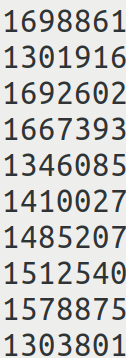
\includegraphics[width=1\textwidth]{slides/images/concurrence_buggy_1.png}
\end{columns}
\end{frame}

\begin{frame}
    Les solutions de synchronisation :
    \begin{itemize}[label=\small\ding{114}]
        \item les opérations atomiques (module \texttt{Atomic}) : une opération qui s'exécute sans être interrompus
        \item les mutex (algorithme de Peterson et de la boulangerie)
        \item les sémaphores
    \end{itemize}
\end{frame}

\begin{frame}[fragile]{Peterson}
    \begin{lstlisting}
    let b1, b2 = Atomic.make false, Atomic.make false
    let tour = Atomic.make 0
    \end{lstlisting}
    \begin{columns}
    \column{0.48\linewidth}    
    \begin{lstlisting}[numbers=left]
      let rec p1 () =
       Atomic.set b1 true;
       Atomic.set tour 2;
       while (Atomic.get b2
        && Atomic.get tour = 2) do () 
        done;
        (* SC *)
       Atomic.set b1 false;
        p1 ()
       
    \end{lstlisting}
    \column{0.50\linewidth}
    \begin{lstlisting}
     let rec p2 () =
      Atomic.set b2 true;
      Atomic.set tour 1;
      while (Atomic.get b1 
        && Atomic.get tour = 1) do () 
      done;
      (* SC *) 
      Atomic.set b2 false;
       p2 ()
    \end{lstlisting}
    \end{columns}
\end{frame}

\begin{frame}{Propriétés de Peterson}
    
    \begin{itemize}[label=\small\ding{114}]
         \item un seul thread peut être dans la section critique en même temps (preuve par l'absurde)
        \item pas d'interblocage : un thread peut toujours avancer
        \item pas de famine : un thread ne peut pas ne jamais avoir accès à la SC
    \end{itemize}
\end{frame}

\begin{frame}[fragile]{Peterson}
\begin{lstlisting}
module Mutex = struct
  type 'a t = 
    { flag : bool Atomic.t Array.t; 
      turn : int Atomic.t }

  let init () =
    { flag = Array.make 2 (Atomic.make false); 
      turn = Atomic.make 0 }

  let lock t id =
    Atomic.set t.flag.(id) true;
    Atomic.set t.turn (1 - id);
    while Atomic.get t.flag.(1 - id) && Atomic.get t.turn = 1 - id do
      ()
    done
    
  let unlock t id = Atomic.set t.flag.(id) false
end
\end{lstlisting}

\end{frame}

\begin{frame}[fragile]{Algorithme de la boulangerie}
\begin{lstlisting}[basicstyle=\scriptsize\ttfamily]
  type t =
    { compteur : int Array.t; choix : bool Array.t; size : int }
    
  let init size =
    { compteur = Array.make size 0; choix = Array.make size false; size} 

  let lock t id =
    t.choix.(id) <- true;
    let max = ref 0 in
    Array.iteri 
        (fun i elt -> if i <> id then max := Int.max elt !max) 
        t.compteur;
    t.compteur.(id) <- !max + 1;
    t.choix.(id) <- false;
    for j = 0 to t.size -1 do
      while t.choix.(j) do () done;
      while t.compteur.(j) > 0 &&
           (t.compteur.(j) < t.compteur.(id) ||
           (t.compteur.(j) == t.compteur.(id) && j < id)) do () done;
    done

  let unlock t id =
    t.compteur.(id) <- 0
end
\end{lstlisting}

\end{frame}
